\documentclass{article}

\usepackage{tikz}

\usetikzlibrary{shapes.geometric, arrows}

\tikzset{
    startstop/.style={rectangle, rounded corners, minimum width=3cm, minimum height=1cm, text centered, draw=black, fill=red!30},
    io/.style={trapezium, trapezium left angle=70, trapezium right angle=110, minimum width=3cm, minimum height=1cm, text centered, draw=black, fill=blue!30},
    process/.style={rectangle, minimum width=3cm, minimum height=1cm, text centered, draw=black, fill=orange!30},
    decision/.style={diamond, minimum width=3cm, minimum height=1cm, text centered, draw=black, fill=green!30},
    arrow/.style={thick, ->, >=stealth}
}

\begin{document}

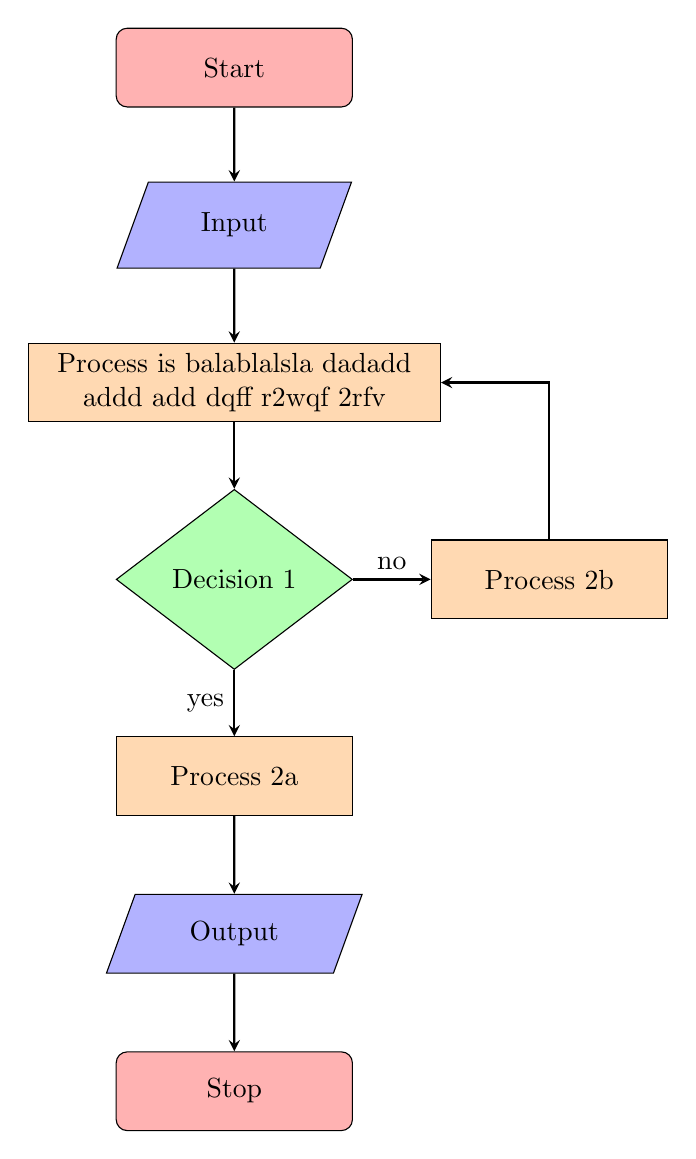
\begin{tikzpicture}[node distance=2cm]
    
    \node (start) [startstop] {Start};
    \node (in1) [io, below of=start] {Input};
    \node (pro1) [process, below of=in1, text width=5cm] {Process is balablalsla dadadd addd add dqff r2wqf 2rfv};
    \node (dec1) [decision, below of=pro1, yshift=-0.5cm] {Decision 1};
    \node (pro2a) [process, below of=dec1, yshift=-0.5cm] {Process 2a};
    \node (pro2b) [process, right of=dec1, xshift=2cm] {Process 2b};
    \node (out1) [io, below of=pro2a] {Output};
    \node (stop) [startstop, below of=out1] {Stop};
    
    \draw [arrow] (start) -- (in1);
    \draw [arrow] (in1) -- (pro1);
    \draw [arrow] (pro1) -- (dec1);
    \draw [arrow] (dec1) -- node[anchor=east] {yes} (pro2a);
    \draw [arrow] (dec1) -- node[anchor=south] {no} (pro2b);
    \draw [arrow] (pro2b) |- (pro1);
    \draw [arrow] (pro2a) -- (out1);
    \draw [arrow] (out1) -- (stop);

\end{tikzpicture}

\end{document}
